\documentclass[12pt]{article}
\usepackage{amsmath}
\usepackage{graphicx}
\graphicspath{ {images/}}
\usepackage[ngerman,english]{babel}
\usepackage{tabularx}  % for 'tabularx' environment and 'X' column type
\usepackage{ragged2e}  % for '\RaggedRight' macro (allows hyphenation)
\newcolumntype{Y}{>{\RaggedRight\arraybackslash}X} 
\usepackage{float}
\restylefloat{table}

%	options include 12pt or 11pt or 10pt
%	classes include article, report, book, letter, thesis

\title{Machine Learning for Applications in Computer Vision: Week 1}
\author{Neeraj Sujan - 03656452 }
\date{23 April 2015}

\begin{document}
\maketitle

Exercise 2: Support Vector Machines
\\

Results:

The training data set is stored in images and labels. The test data set is stored in images1 and labels1. The tests were carried out for the first 1000 samples using linear kernel,polynomial kernel and RBF kernel. The results of the tests are given below. 

I got the best performance using the polynomial and linear kernel whereas for the RBF kernel, I got the worst performance. The performance metric is as displayed below \\

\begin{table}[h]
\centering
\begin{tabular}{|c|c|c|c|c|}
\hline 
Classifier & LinearSVC & SVC,linear kernel & SVC,polynomial kernel & SVC,RBF kernel \\ 
\hline 
Accuracy & 0.8235 & 0.8758 & 0.8865 & 0.1028 \\ 
\hline 
\end{tabular} 
\end{table}

\begin{figure}[h]
\centering
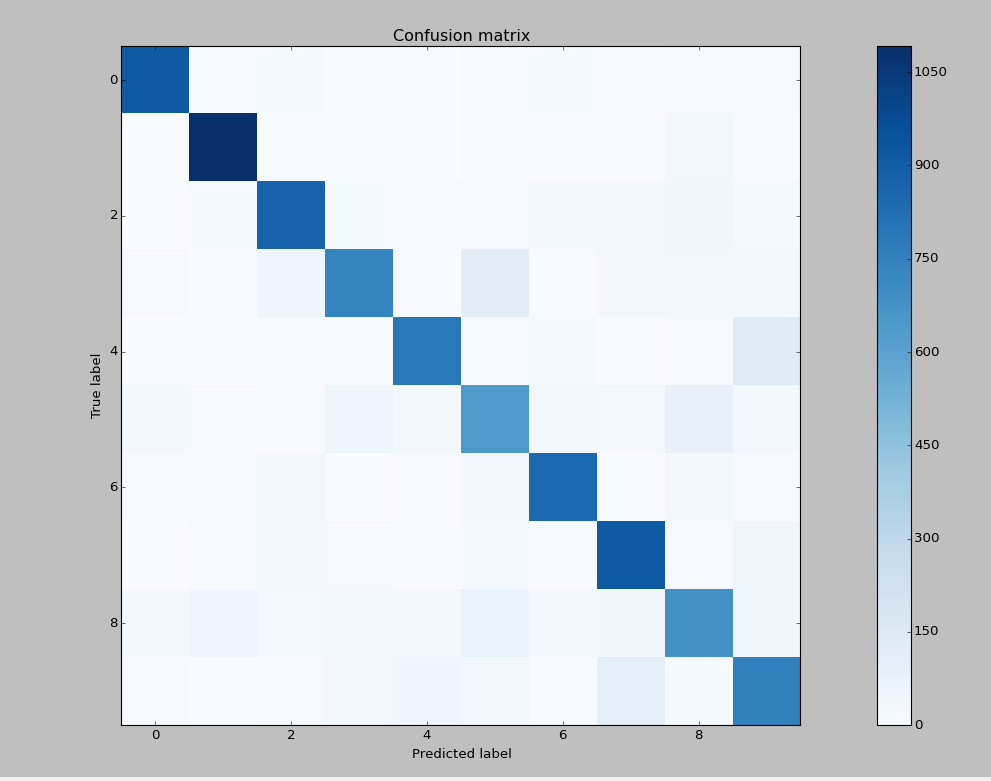
\includegraphics[width=10cm, height=4cm]{1}
\end{figure}

\begin{figure}[h]
\centering
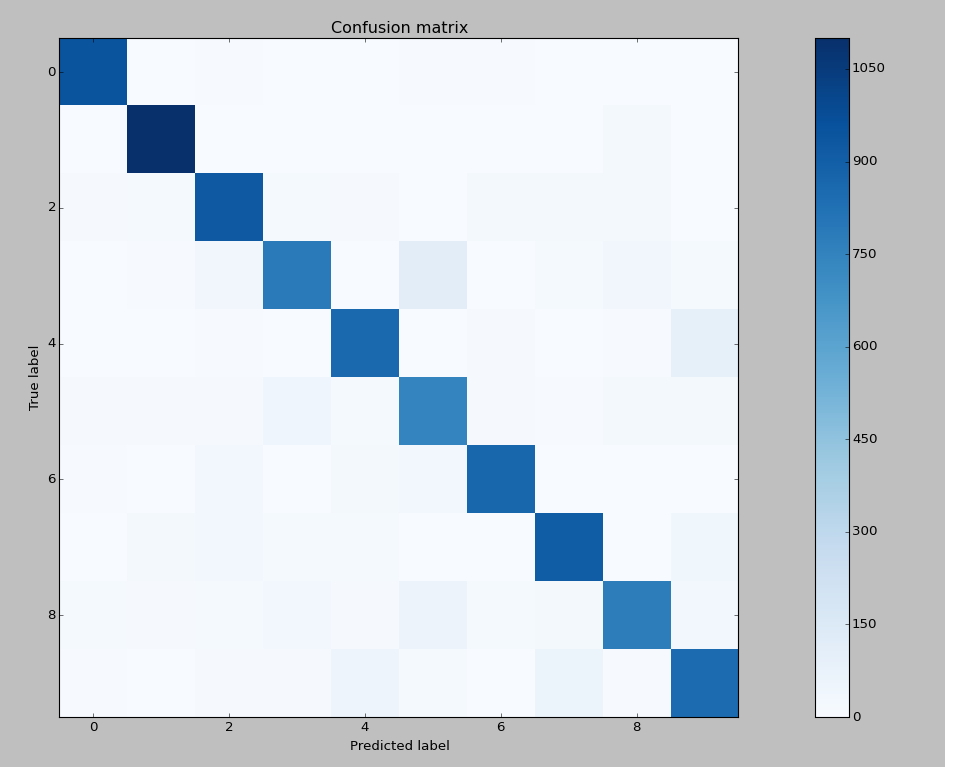
\includegraphics[width=10cm, height=4cm]{2}
\end{figure}

\begin{figure}[h]
\centering
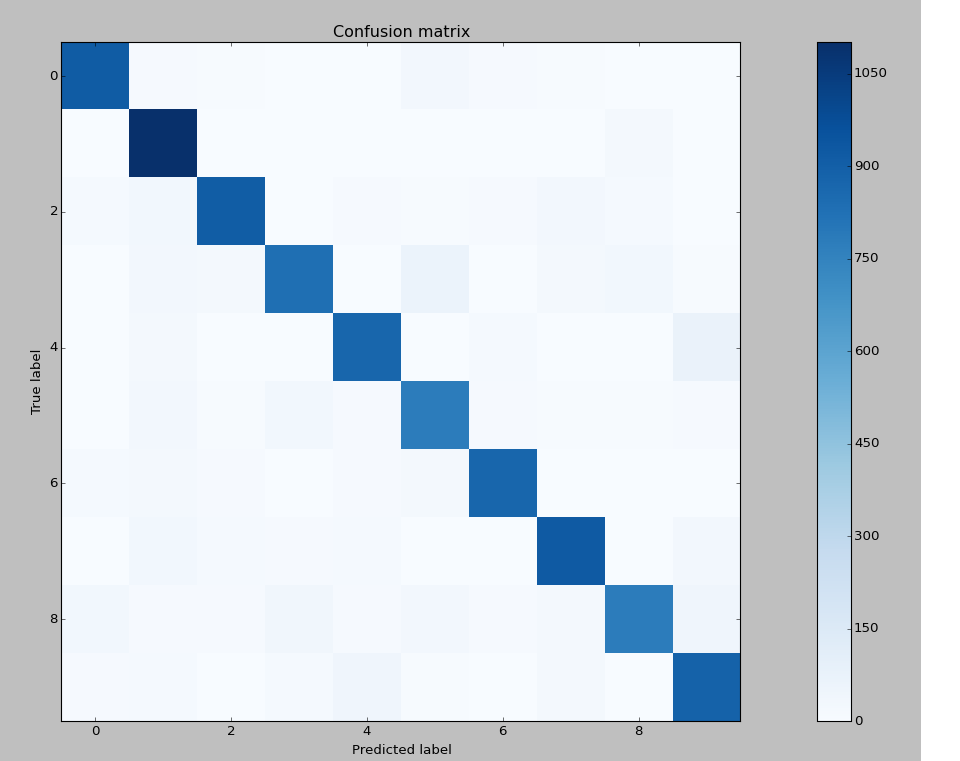
\includegraphics[width=10cm, height=4cm]{3}
\end{figure}
\begin{figure}[h]
\centering
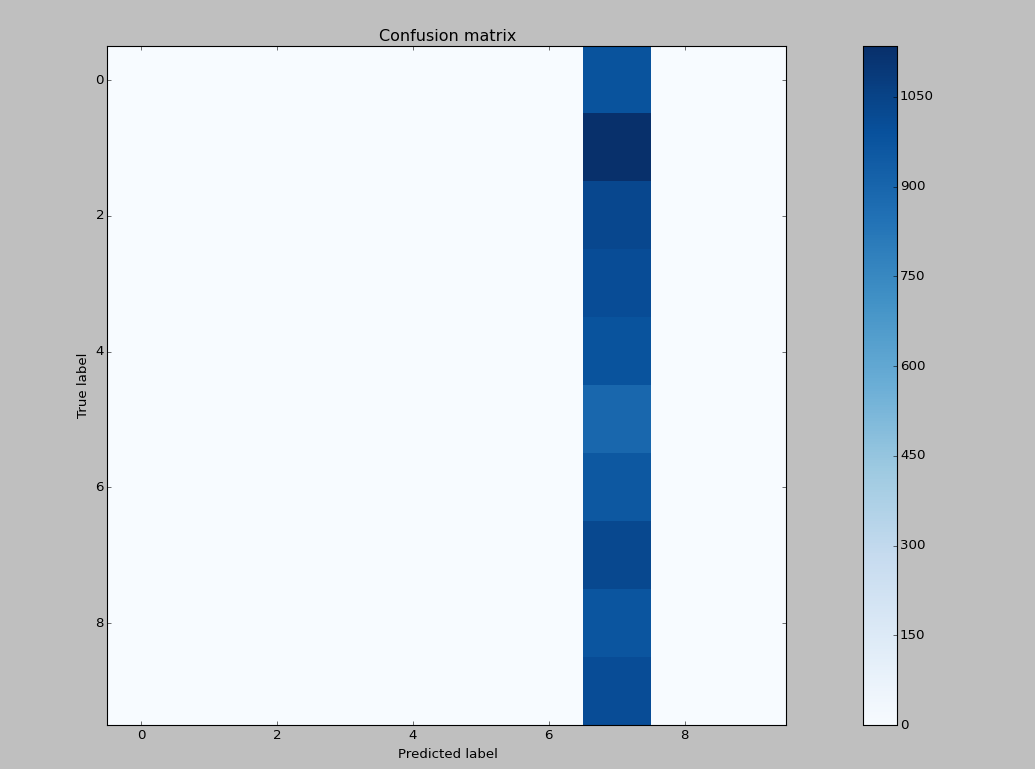
\includegraphics[width=10cm, height=4cm]{4}
\end{figure}

\newpage

\end{document}
